\begin{itemize}
\item Togglable button to turn each page into a \,flashcard\,.
\item Internal \ref{aboutme|links|Used to demonstrate an internal link} (and lists of pages that link to current page)
\item Tags, represented by colors: \begin{itemize}
	\item \textcolor{green}{Definitions}
	\item \textcolor{purple}{Propositions}
	\item \textcolor{red}{Exercises}
	\item \textcolor{blue}{Examples}
	\item \textcolor{pink}{Kris' commentary}
	\end{itemize}
\item Content written in \LaTeX: $1+\frac{\phi}{sin(\psi)}$
\item Foot\footnote{notes}
\item Citations \cite{mazieres2005get}
\item TikZ: \begin{tikzcd}
	A & B \\
	& C
	\arrow["f", from=1-1, to=1-2]
	\arrow["g", from=1-2, to=2-2]
	\arrow["{f;g}"', dashed, from=1-1, to=2-2]
\end{tikzcd}\
\item Images: 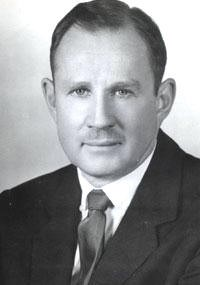
\includegraphics{sellars-w.jpeg}

\end{itemize}

Built from Haskell (\href{https://github.com/kris-brown/KBKB}{source code}).
